\subsection{小数据量}
以下展示基于题目提供的课程信息json文件,文件系统部分使用Python中的Pandas库处理。
\begin{lstlisting}[language=python]
@timer
def db_query():
    for _ in range(10):
        cur.execute('''SELECT DISTINCT cid
                       FROM project1.course
                       WHERE credit > 2;''')
    print(len(cur.fetchall()))

@timer
def fs_query():
    result_set = set()
    for _ in range(10):
        result_set.clear()
        for index, c in cif.iterrows():
            if c['courseCredit'] > 2:
                result_set.add(c['courseId'])
    print(len(result_set))
\end{lstlisting}
\vspace{-2em}
\par 上例重复十次查询所有计算机系开设的课程的列表,数据库耗时0.298s,文件系统耗时0.296s,可见即使是在运行速度较慢的Python中,依然能以微弱的优势领先数据库。这是由于小文件的遍历开销相对不大,而对于数据库的每次查询都有对任务的优化规划、SQL的语法检查、用户权限检查等环节的额外开销,因此查询耗时总耗时接近甚至超过文件系统的查询。

\par
数据库的安全性及完善的检查机制是文件系统所远不能及的,但也正是其一系列复杂的流程(语法检查、权限验证)为查询带来了一定的额外开销。当数据量大时,此开销相比于查询开销的比例极小,可以忽略不计,且一系列的优化(哈希、缓存、并行等)大大提升了查询效率;而对于极小的数据量,直接遍历文件已经作为较优的解决方案,DBMS在规划后可能给出的也是Seq scan的方案,但上述额外开销反而导致耗时较多。但从实际应用中来讲,应用数据库所存储的信息一般至少上千条,且查询的分摊总条目数也远大于遍历依然能跑赢优化的边界数量,也即平均角度上,使用数据库的查询性能是远优于文件系统的;且现实应用离不开数据库带来的一系列完善的检查及权限机制,数据库的优势依然是文件系统无法比拟的。\\~\\
\centerline{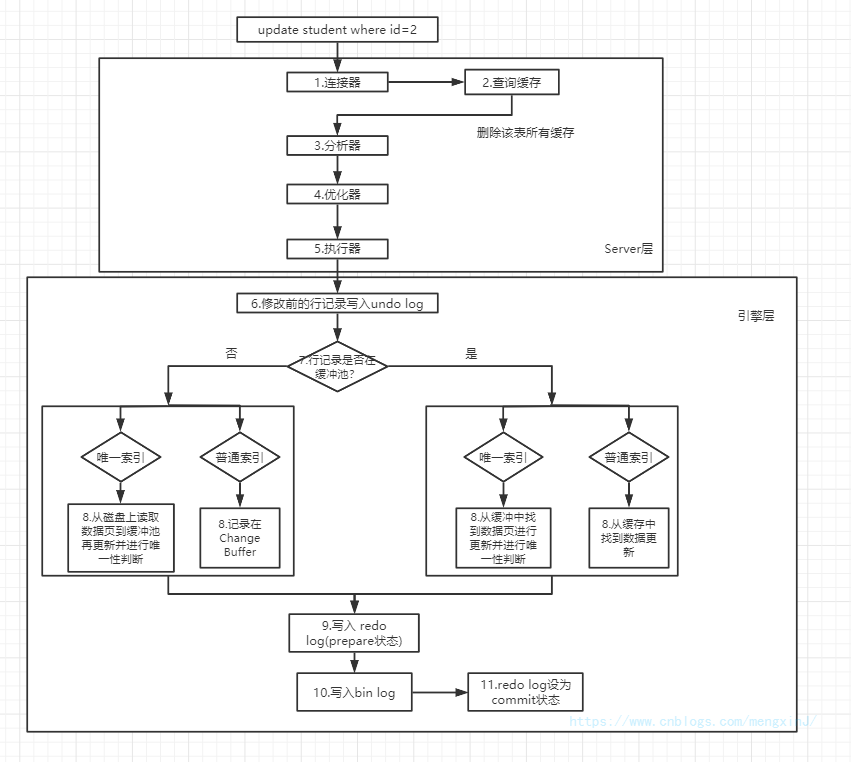
\includegraphics[width=0.8\textwidth]{pic/qry}}
\scriptsize
\centerline{InnoDB存储引擎的SQL操作过程\textsuperscript{\cite{m-2020}}}
\normalsize